\section{Processi di supporto}


\subsection{Documentazione}
\label{sec:documentazione}
\subsubsection{Scopo}
L'attività di documentazione consiste nella redazione di documenti durante tutto il ciclo di vita del prodotto software. Il gruppo si impegna a rispettare ed applicare le norme e gli strumenti adottati, con l'obiettivo di garantire una stesura senza ambiguità di una documentazione valida, coerente e conforme a delle precise regole. 

\subsection{Attività}

\paragraph{Stesura} \Spazio 
I documenti vengono redatti secondo le norme definite nella sezione \ref{struttura} 

\paragraph{Approvazione dei documenti} \Spazio
Ogni documento non formale in corrispondenza del completamento della sua stesura dovrà essere sottoposto al \textit{Project Manager}, che dovrà delegare ai \textit{Verificatori} il controllo del contenuto e della forma. Nel caso gli anzidetti \textit{Verificatori} rilevino degli errori, sarà loro compito notificarli al \textit{Project Manager}, che a sua volta affiderà al redattore del documento il compito di correggerli. Questo ciclo va eseguito fino a quando il documento non viene considerato completamente corretto dai  \textit{Verificatori}. In caso di assenso sulla correttezza e sulla qualità il documento può essere reputato un documento formale. In caso contrario spetta al \textit{Project Manager} comunicare le ragione per cui il documento non è stato giudicato corretto, esplicitando le modifiche da apportare.

\paragraph{Aggiornamento} \Spazio 
I documenti prodotti non possono essere completi fin dall'inizio per questo essi vanno aggiornati in concomitanza con lo sviluppo del progetto, in particolare il documento \textit{Norme di Progetto} deve essere incrementato al fine di normare tutte le attività non previste o le cui norme precedentemente individuate non si adattino alle esigenze del gruppo e del progetto. 


\subsubsection{Template}
Per agevolare la redazione della documentazione è stato creato un template \LaTeX\text{ } contenente tutte le impostazioni stilistiche e grafiche citate in questo documento.

\subsubsection{Struttura dei documenti}
\label{struttura}

\paragraph{Prima pagina}\Spazio
Ogni documento, esclusi i verbali, è caratterizzato da una prima pagina che contiene le seguenti informazioni sul documento:
\begin{itemize}
	\item Logo del gruppo;
	\item Titolo del documento;
	\item Nome del gruppo;
	\item Nome del progetto;
	\item Versione del documento;
	\item Nome e cognome dei redattori del documento;
	\item Nome e cognomedei verificatori del documento;
	\item Nome e cognome del responsabile approvatore del documento;
	\item Destinazione d’uso del documento;
	\item Lista di distribuzione del documento;
	\item Una breve descrizione del documento.
\end{itemize}

\paragraph{Diario delle modifiche} \Spazio
\label{registroModifiche}
La seconda pagina di ogni documento contiene il diario delle modifiche del documento.
Ogni riga del diario delle modifiche contiene:
\begin{itemize}
	\item Un breve sommario delle modifiche svolte;
	\item Nome e cognome dell’autore;
	\item Ruolo dell’autore;
	\item Data della modifica;
	\item Versione del documento dopo la modifica.
\end{itemize}
La tabella contenente le modifiche è ordinata per data in ordine decrescente, affinchè la prima riga contenga la versione attuale del documento.

\paragraph{Indici} \Spazio
In ogni documento, esclusi i verbali, è presente un indice delle sezioni, un indice delle figure e un indice delle tabelle. Nel caso non siano presenti figure o tabelle i rispettivi indici verranno omessi. La notazione numerica di ogni indice deve partire da 1 e le sottosezioni devono essere separate da un punto. Anche la notazione della sottosezione parte da 1.

\paragraph{Formattazione generale delle pagine} \Spazio
Il template prevede dei margini orizzontali e verticali che devono essere rispettati in ogni pagina. Ad esclusione della prima, tutte le pagine contengono un’intestazione ed un piè di pagina.

\subparagraph{Intestazione} \Spazio
L’intestazione è così strutturata:
\begin{itemize}
	\item Logo del gruppo posto a sinistra;
	\item Indirizzo di posta elettronica del gruppo posto a destra.
\end{itemize}

\subparagraph{Piè di pagina} \Spazio
Il piè di pagina è così strutturato:
\begin{itemize}
	\item Nome del documento corrente, posto a sinistra;
	\item Numerazione progressiva della pagina rispetto al totale posta a destra.
\end{itemize}

\paragraph{Note a piè di pagina} \Spazio
In caso di presenza in una pagina interna di note da esplicare, esse vanno indicate nella pagina corrente, in basso a sinistra. Ogni nota deve riportare un numero e una	descrizione.

\subsubsection{Versionamento}
\label{versionamento}
Tutti i documenti, esclusi i verbali, devono essere versionati, affinchè si possa in ogni momento conoscerne la storia. Ogni versione di un documento deve essere appuntata nel Diario delle Modifiche. Si deve adottare il seguente formato per registrare ogni modifica:
\textbf{v{X}.{Y}.{Z}}
dove:
\begin{itemize}
	\item \textbf{X}
	      \begin{itemize}
		      \item Parte da 0;
		      \item Viene incrementato dal \textit{Project Manager} in concomitanza con l'approvazione del documento;
		      \item Arriva fino al numero di revisioni a cui è sottoposto il docuemnto.
	      \end{itemize}

	\item \textbf{Y}
	      \begin{itemize}
		      \item Parte da 0;
		      \item Viene incrementato dal \emph{Verificatore} in concomitanza di ogni verifica oppure dal \emph{Redattore} in concomitanza con la stesura di una modifica corposa, come l'aggiunta di una sezione;
		      \item Quando X viene incrementato Y ritorna a 0.
	      \end{itemize}

	\item \textbf{Z}
	      \begin{itemize}
		      \item Parte da 0;
		      \item Viene incrementato dal \textit{Redattore} in concomitanza di ogni modifica di piccolo volume, come la correzione di alcuni errori;
		      \item Quando Y viene incrementato Z	 ritorna a 0.
	      \end{itemize}

\end{itemize}

\subsubsection{Norme tipografiche}
Per la redazione della documentazione bisogna attenersi alle seguenti norme.

\paragraph{Stile del testo}
\begin{itemize}
	\item \textbf{Grassetto:} il grassetto può essere utilizzato nei seguenti casi:
	      \begin{itemize}
		      \item \textbf{Elenchi puntati:} in questi casi può essere utilizzato il grassetto per evidenziare il concetto sviluppato nella continuazione del punto;
		      \item \textbf{Altri casi:} per evidenziare particolari passaggi o parole chiave.
	      \end{itemize}

	\item \textbf{Corsivo:} il corsivo deve essere utilizzato nei seguenti casi:
	      \begin{itemize}
		      \item \textbf{Citazioni:} quando si deve citare una frase questa va scritta in corsivo;
		      \item \textbf{Abbreviazioni:} quando possibile si deve preferire una parola completa ad un’abbreviazione;
		      \item \textbf{Nomi particolari:} il corsivo deve essere utilizzato quando si parla di figure particolari (es. \textit{Progettista});
		      \item \textbf{Documenti:} il corsivo deve essere utilizzato quando si parla di documenti (es.\textit{Glossario});
		      \item \textbf{Altri casi:} in altre situazione, il corsivo va utilizzato per mettere in rilievo passaggi o parole significativi, evidenziare riferimenti ai documenti interni o esterni.
	      \end{itemize}

	\item \textbf{Maiuscolo:} l’utilizzo di parole completamente in maiuscolo è riservato solo agli acronimi.

\end{itemize}

\paragraph{Elenchi puntati} \Spazio
Ogni punto dell’elenco deve terminare con un punto e virgola,tranne l’ultimo che deve terminare con un punto. La prima parola deve avere la lettera maiuscola, a meno di casi particolari (e.g. nome di un file);

\paragraph{Formati comuni} \Spazio
\label{formati}
Per rappresentare le seguenti entità vanno usate le seguenti modalità:
\begin{itemize}

	\item \textbf{Orari:}
	      \textbf{HH:MM}
	      \begin{itemize}
		      \item \textbf{HH:} va da 0 a 23 e rappresenta l'ora;
		      \item \textbf{MM:} va da 0 a 59 e rappresenta i minuti.
	      \end{itemize}

	\item \textbf{Date:}
	      \textbf{AAAA-MM-GG}
	      \begin{itemize}
		      \item \textbf{AAAA:} rappresenta l'anno;
		      \item \textbf{MM:} rappresenta il mese;
		      \item \textbf{GG:} rappresenta il giorno.
	      \end{itemize}

	\item \textbf{Termini ricorrenti:}
	      \begin{itemize}
		      \item \textbf{Nomi proprio:} ogni nome proprio va scritto con il formalismo \textit{Nome Cognome};
		      \item \textbf{Ruoli di progetto:} ogni ruolo va scritto con l'iniziale maiuscola e in corsivo;
		      \item \textbf{Nomi dei documenti:} ogni documenti va scritto con l'iniziale maiuscola e in corsivo.
	      \end{itemize}

\end{itemize}

\paragraph{Sigle} \Spazio
È previsto l’utilizzo delle seguenti sigle:
\begin{itemize}
	\item AR: \textit{Analisi dei Requisiti};
	\item PP: \textit{Piano di Progetto};
	\item NP: \textit{Norme di Progetto};
	\item SF: \textit{Studio di Fattibilità};
	\item PQ: \textit{Piano di Qualifica};
	\item TB: \emph{Technology Baseline};
	\item PB: \emph{Produce Baseline}.
	\item RR: \emph{Revisione dei requisiti};
	\item RP: \emph{Revisione di progettazione};
	\item RQ: \emph{Revisione di qualifica};
	\item RA: \emph{Revisione di accettazione};
\end{itemize}

\subsubsection{Elementi grafici}
\paragraph{Tabelle}\Spazio
Le tabelle presenti all'interno del documento devono essere centrate orizzontalmente nella pagina e devono presentare una didascalia sottostante avente un indice identificativo univoco incrementale per agevolarne il tracciamento, oltre che una breve descrizione del loro contenuto.\\
Le tabelle del diario delle modifiche invece non hanno alcuna descrizione.
Qualora il redattore lo ritenesse necessario per aumentare la leggibilità è possibile anche l'uso di colori di sfondo scegliendone uno specifico per l'intestazione e due che verranno alternati per le righe sottostanti.

\paragraph{Immagini}\Spazio
Le immagini inserite nel documento devono essere nel formato \gl{PNG}. Ognuna di esse deve essere accompagnata da una didascalia analoga a quella descritta per le tabelle. \\
Ogni immagine deve inoltre essere centrata orizzontalmente mantenendo una separazione netta dai paragrafi che seguono e precedono, marcando quindi un distacco tra grafica e testo migliorando di conseguenza la leggibilità. \\
I diagrammi UML vengono inseriti nei documenti sotto forma di immagine.
\subsubsection{Classificazione dei documenti}
\paragraph{Documenti informali}\Spazio
Tutti i documenti sono informali dalla loro creazione fino all'approvazione da parte del \emph{Project Manager} ed in quanto tali sono considerati esclusivamente ad uso interno.
\paragraph{Documenti formali}\Spazio
Una volta avvenuta l'approvazione da parte del \emph{Project Manager} il documento viene ritenuto formale ed è quindi distribuibile all'esterno del gruppo.\\
Per raggiungere tale stato inoltre, il documento deve aver già superato la fase di verifica. \\
Ogni modifica effettuata produrrà una nuova versione del documento da considerarsi informale e rimarrà tale fino ad una successiva approvazione da parte del \emph{Project Manager}.
\paragraph{Verbali}\Spazio
\label{verbali}
Dopo ogni incontro interno o esterno spetta al segretario verbalizzante redigere il documento. I verbali non sono soggetti a versionamento poiché non subiscono modifiche successive alla loro prima redazione. Deve avere un codice univoco identificativo con la seguente struttura:
\newline
\centerline{V*\_[data]}
dove:
\begin{itemize}
	\item \textbf{data} è la data della riunione alla quale il verbale fa riferimento nel formato descritto in \ref{formati};
	\item \textbf{*} è o la lettera I se il verbale è interno, oppure la lettera E se il verbale è esterno.
\end{itemize}
Dovrà presentare le seguenti informazioni nell'ordine in cui sono elencate:
\begin{itemize}
	\item luogo dell'incontro, data e ora;
	\item partecipanti presenti, assenti, il nome di chi presiede e quello del segretario verbalizzante.
\end{itemize}
Tali informazioni devono essere contenute nel primo paragrafo \textit{Informazioni Generali}, che deve specificare anche gli argomenti trattati durante l'incontro.\\
Il secondo paragrafo \textit{Argomenti Affrontati} deve esplicitare in dettaglio le decisioni prese o i problemi irrisolti.\\
Nel caso l'incontro abbia partecipanti esterni e fosse stata eseguita una serie di domande e risposte deve essere presente una sezione  \textit{Domande e Risposte} dove vengono riportate le domande poste, seguite dalle risposte date.
\subsubsection{Strumenti}
\label{sec:strumentips}
\paragraph{\LaTeX}\Spazio
Per redigere i documenti viene utilizzato il linguaggio di markup \LaTeX. La possibilità di definire delle variabili all'interno dei fogli di stile consente di automatizzare l'aggiornamento di tutti i riferimenti presenti all'interno dei diversi documenti.\\
Inoltre permette la creazione di documenti formali e divisi in sezioni molto velocemente, potendo separare il contenuto dalla formattazione tramite un file template separato e condiviso da tutti i documenti.\\
Infine grazie all'elevato numero di librerie, permette di avere un'alta personalizzazione del documento.
\paragraph{TexStudio}\Spazio
L'editor scelto per sviluppare i documenti in \LaTeX\text{ } è \gl{TexStudio} nella versione 2.12.6.
Lo strumento multipiattaforma integra un compilatore e un visualizzatore PDF, fornendo anche suggerimenti per completare i comandi \LaTeX.
\begin{figure}[H]
	\centering
	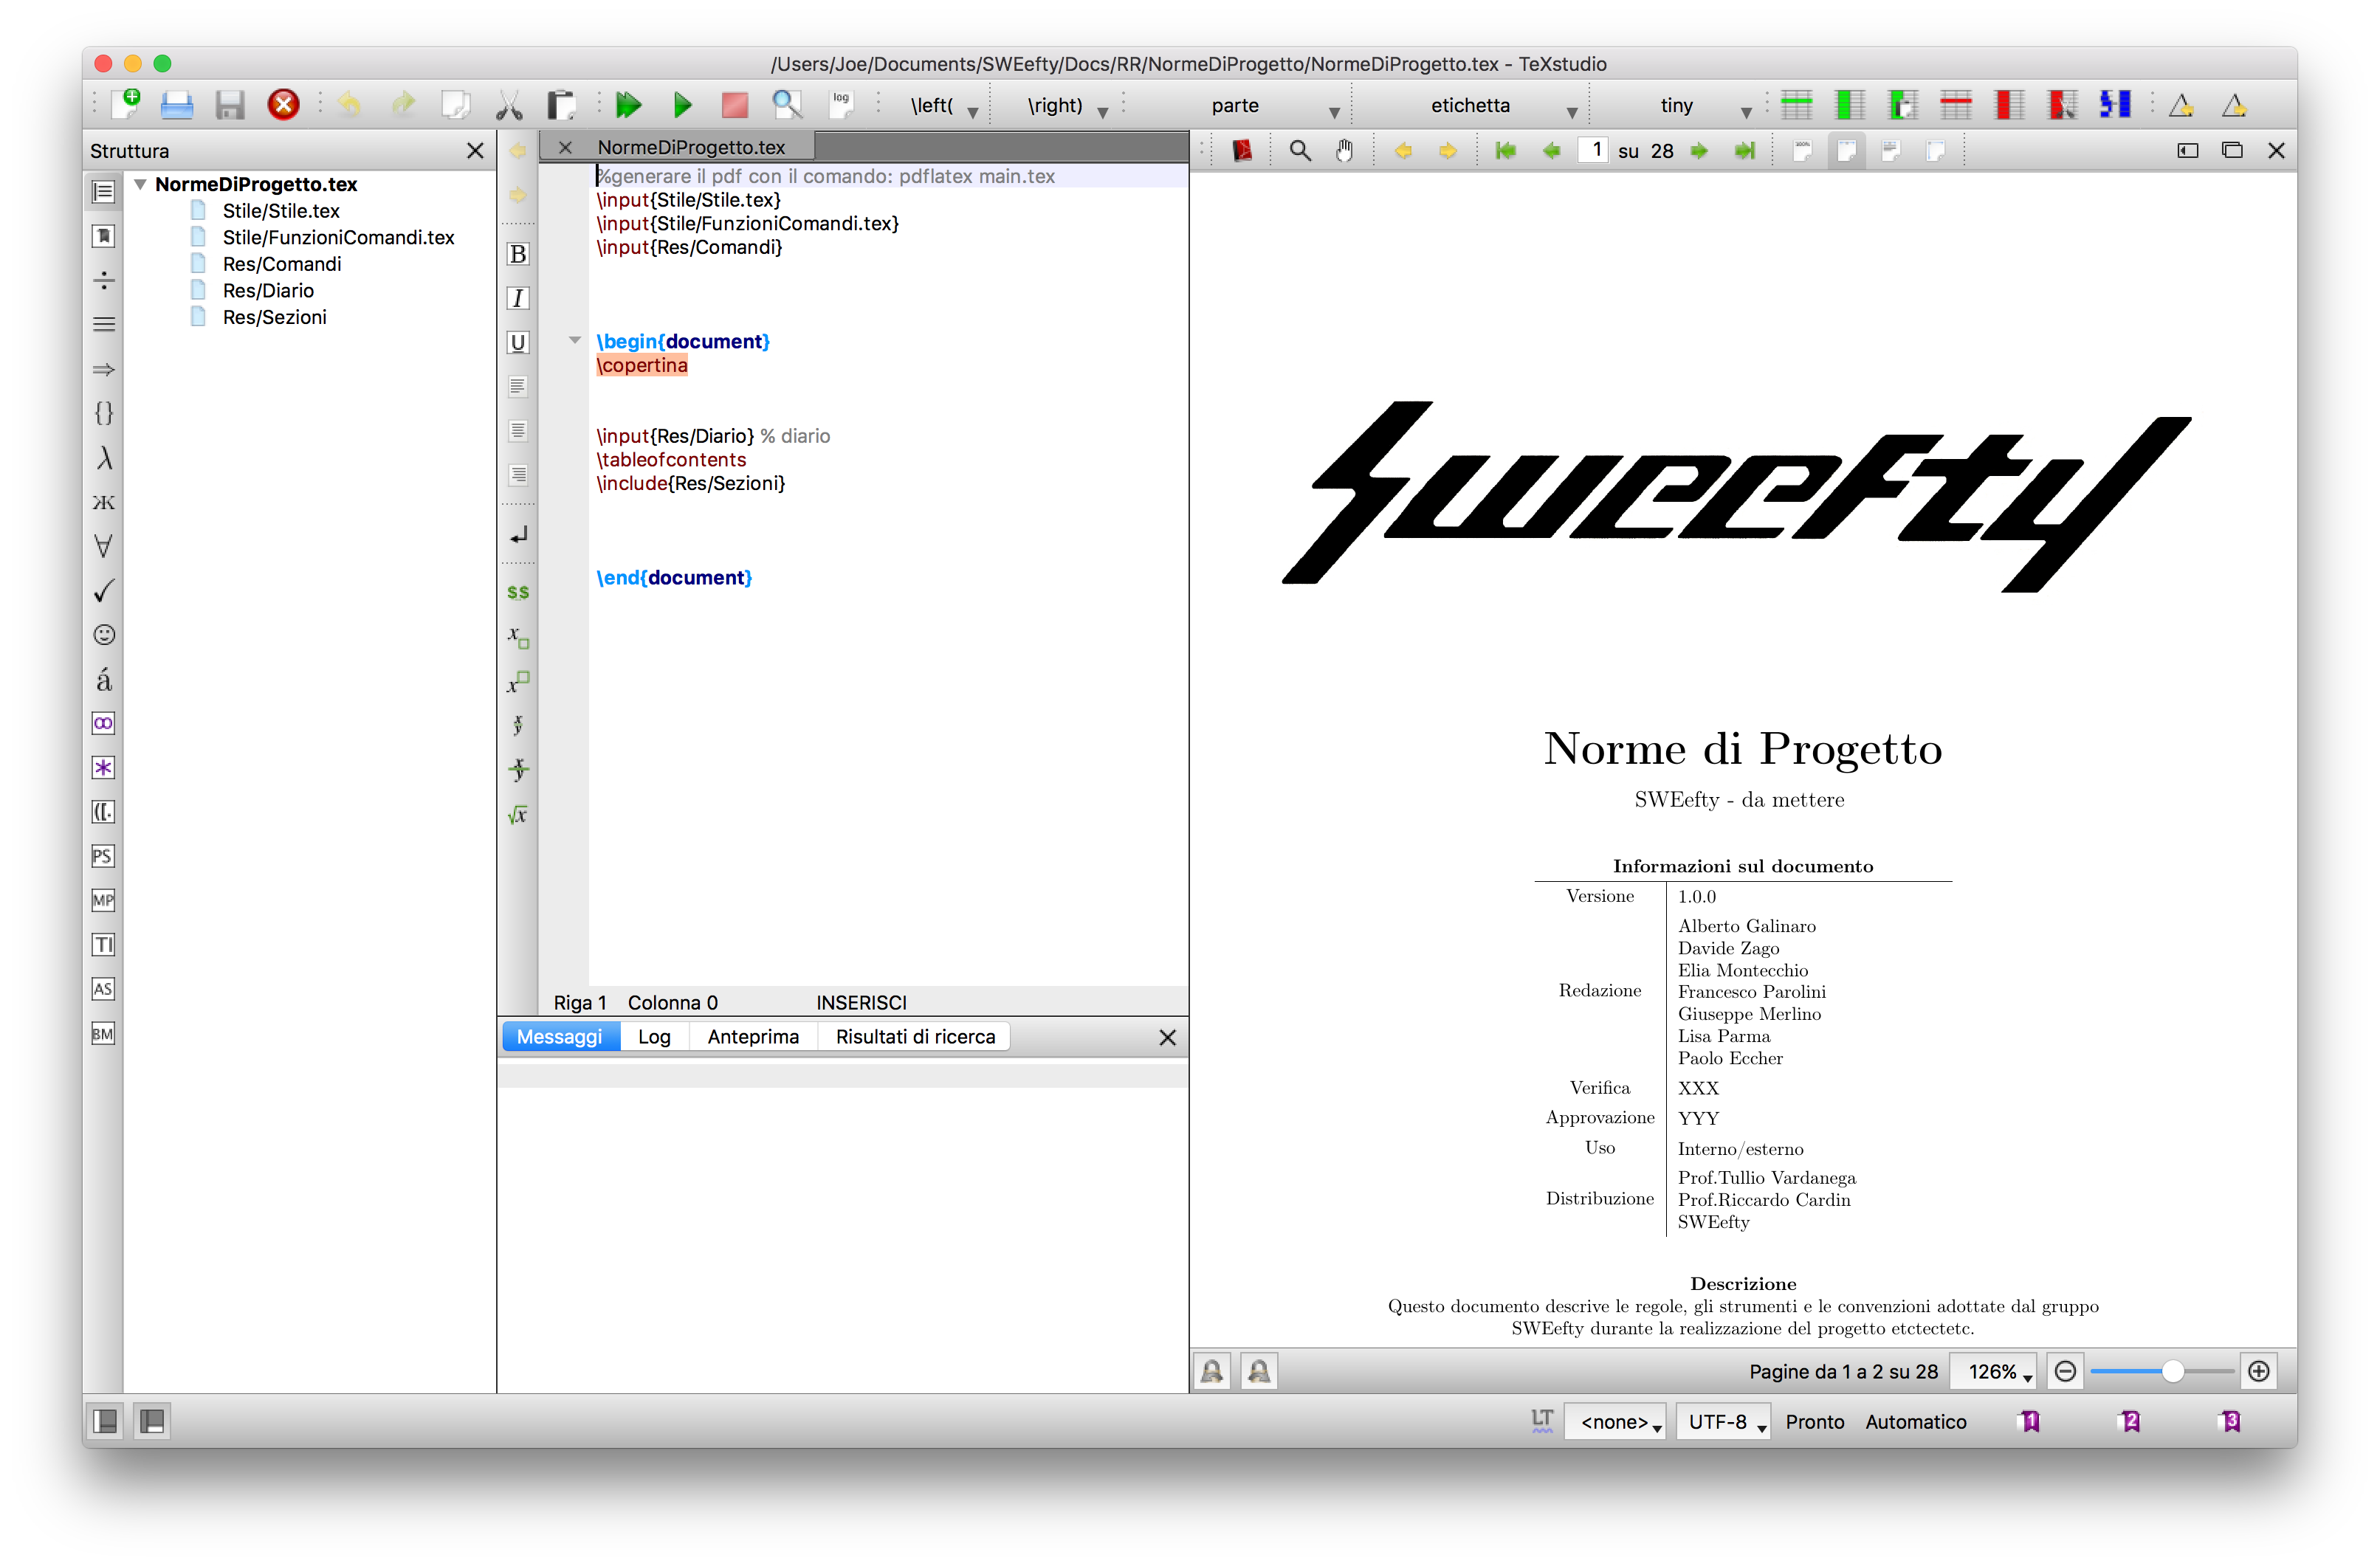
\includegraphics[width=1\textwidth]{Images/texstudio.png}
	\caption{TexStudio in versione desktop per Mac OSX}
\end{figure}

\subsection{Verifica}
\label{sec:verificaps}

\subsubsection{Scopo}
La verifica accerta che l'esecuzione delle attività di processo attuate nel periodo in esame non abbia introdotto errori fornendo una prova oggettiva che dimostri di aver soddisfatto i requisiti definiti per i processi analizzati.
Inoltre, si esamina la consistenza, completezza e correttezza del software prodotto e/o della documentazione redatta.
\subsubsection{Attività}
\paragraph{Analisi}
\subparagraph{Analisi statica} \Spazio
L'analisi statica è una tecnica utilizzata per identificare errori all'interno di documenti e del codice sorgente, senza la necessità eseguirlo, è applicabile durante tutto il loro ciclo di vita in due diverse modalità:
\begin{itemize}
	\item \textbf{Walkthrough}:
	      consiste nel leggere il documento/codice cercando anomalie senza avere un'idea chiara di che tipo di errori possono essere trovati, è un'attività onerosa e non efficiente ma necessaria durante le prime fasi di progetto dove sarà la principale forma di verifica adottata, in quanto non è chiaro fin dall'inizio che tipo di errori si possono fare.
	      Vista la sua scarsa efficacia normalmente viene effettuata da più persone.
	\item \textbf{Inspection}:
	      consiste nella lettura mirata del documento/codice per localizzare possibili errori specificati dalla lista di controllo. Ha un basso costo e diventa più efficace con l'esperienza e l'estensione della lista di controllo, per questo può essere effettuata da una persona sola.
\end{itemize}
Ogni errore rilevato va discusso con l'autore allo scopo di concordare una modifica.
\subparagraph{Analisi dinamica} \Spazio
L'analisi dinamica è una forma di analisi del software che richiede l'esecuzione del codice sorgente. Viene effettuata tramite dei test che verificano il corretto funzionamento del prodotto, in caso di anomalie questi test aiutano ad identificare l'errore.
I test devono essere ripetibili ovvero con lo stesso input e nello stesso ambiente devo essere in grado di ottenere sempre lo stesso output. Per ogni test sono quindi definiti i seguenti parametri:
\begin{itemize}
	\item \textbf{Ambiente}: sistema hardware e software sul quale si svolgerà il test;
	\item \textbf{Stato iniziale}: insieme dei valori assunti dalle variabili dinamiche prima dello svolgimento dei test;
	\item \textbf{Input}: i valori di ingresso specificati in ciascun caso di prova;
	\item \textbf{Output}: esito decidibile verificato rispetto a un comportamento atteso;
	\item \textbf{Istruzioni aggiuntive}: istruzioni su come va eseguito il test e su come vanno interpretati gli output.
\end{itemize}
\subsubsection{Metriche}
\label{sec:metriche}
Per garantire la qualità del lavoro di gruppo in questa sezione vengono identificate delle metriche che verranno utilizzate per mantenere sotto controllo la qualità del progetto mentre i correlati obbiettivi di qualità vengono riportati in \textit{Piano di Qualifica v3.0.0} 
\paragraph{Metriche per la qualità di processo} \Spazio
Queste metriche vengono utilizzate per mantenere sotto controllo le variabili critiche del progetto ovvero tempi e costi, e per controllare che la codifica segua alcuni principi di base. 

\subparagraph{Schedule variance} \Spazio
Fornisce una misura di quanto lo stato del progetto è in ritardo o in anticipo rispetto alla pianificazione delle attività.

\textbf{Misurazione: }$SV = BCWP - BCWS$ dove il minuendo indica le attività svolte finora ed il sottraendo le attività che dovrebbero essere svolte finora.


\subparagraph{Cost variance} \Spazio
Indica se si è speso più o meno di quanto è stato previsto.

 \textbf{Misurazione: }$CV = BCWS - ACWP$, il minuendo indica il costo pianificato delle attività svolte ad una certa data ed il sottraendo il costo effettivo delle attività svolte a tale data.

\subparagraph{Rischi non individuati} \Spazio
Indice del numero di rischi non individuati nella fase di analisi:
\textbf{Misurazione: }$SV = BCWP - BCWS$, il minuendo indica le attività svolte finora ed il sottraendo le attività che dovrebbero essere state svolte finora.

\subparagraph{Requisiti obbligatori soddisfatti} \Spazio
Indica quanti requisiti obbligatori sono stati soddisfatti.

\textbf{Misurazione:} $P=100\times\frac{N_S}{N_O}$ dove $N_S$ sono i requisiti soddisfatti, $N_O$ sono i requisiti obbligatori mentre $P$ è la percentuale dei requisiti obbligatori soddisfatti.

\subparagraph{Structural fan-in - SFIN} \Spazio
Indice di utilità da massimizzare, misura il numero di componenti che utilizzano un dato modulo, un valore alto denota un alto riutilizzo del codice.

\subparagraph{Structural fan-out - SFOUT} \Spazio
Indice di dipendenza da minimizzare, misura quante componenti vengono utilizzate dalla componente in esame, un valore alto denota un alto accoppiamento.

\subparagraph{Metodi per classe} \Spazio
Indica il numero di metodi definiti in una classe.

\subparagraph{Parametri per metodo} \Spazio
Indica il numero di parametri passati ad un metodo.

\subparagraph{Complessità ciclomatica} \Spazio
Metrica software utilizzata per misurare la complessità di un programma, misura il numero di cammini linearmente indipendenti attraverso il grafo di controllo di flusso.

\subparagraph{Linee di codice per linee di commento} \Spazio
Misura la percentuale di linee di commento presenti all'interno del codice di un programma.
\textbf{Misurazione:} $P=100\times\frac{N_C}{N_{SLOC}}$ dove $N_C$ è il numero di linee di commento e $N_{SLOC}$ è il numero di linee di codice prodotte.

\subparagraph{Indice Gulpease} \Spazio
L'Indice Gulpease è un indice di leggibilità di un testo tarato sulla lingua italiana, per il suo calcolo vengono considerate due variabili linguistiche: la lunghezza delle parole e la lunghezza delle frasi rispetto al numero delle lettere.
\textbf{Misurazione:} $G=89+\frac{300\times N_F-10\times N_L}{N_P}$ dove $N_F$ è il numero delle frasi, $N_L$ è il numero di lettere e $N_P$ è il numero di parole nel testo.

\subparagraph{Branch coverage}  \Spazio
Misura della percentuale di rami decisionali percorsi dai test dinamici.
\textbf{Misurazione:} $BC=\frac{R_P}{R_T}\times 100$ dove $R_P$ è il numero di rami decisionali percorsi dai test mentre $R_T$ è il numeri di rami decisionali totali presenti nel software.

\subparagraph{Statement coverage} \Spazio
Misura la percentuale linee di codice eseguite almeno una volta dai test dinamici.
\textbf{Misurazione:} $SC=\frac{L_E}{L_T}\times 100$ dove $L_E$ è il numero di linee di codice eseguite almeno una volta dai test mentre $L_T$ è il numero di linee di codice totali all'interno del software.

\paragraph{Metriche per la qualità di prodotto}	\Spazio
Le metriche contenute in questa sezione vengono utilizzate dal gruppo per tenere sotto controllo la qualità del prodotto sviluppato.

\subparagraph{Completezza dell'implementazione funzionale}\Spazio
Misura la quantità in percentuale di requisiti funzionali soddisfatti dalla corrente implementazione.
\textbf{Misurazione:}  $BC=1-\frac{N_{FM}}{N_{FI}}\times 100$, dove $N_{FM}$  è il numero di funzionalità mancanti nell'implementazione e $N_FI$ è il numero di funzionalità individuate nell'attività di analisi.

\subparagraph{Densità di failure} \Spazio
Misura la quantità percentuale di test che si sono conclusi con una failure.
\textbf{Misurazione:} $F=\frac{N_{FR}}{N_{TE}}\times 100$, dove $N_{FR}$ è il numero di failure rilevati durante l'attività di testing e ${N_TE}$ è il numero di test-case eseguiti.

\subparagraph{Comprensibilità delle funzionalità offerte} \Spazio 
Misura la quantità in percentuale di operazioni comprese dall'utente che non richiedono la consultazione del manuale.
\textbf{Misurazione:} $C=\frac{N_{FC}}{N_{FO}}\times 100$, dove $N_{FC}$ è il numero di funzionalità comprese in modo immediato dall'utente e $N_{FO}$ è il numero di funzionalità totali offerte dal sistema.
 
\subparagraph{Facilità di apprendimento} \Spazio 
Misura il tempo medio che occorre ad un utente per imparare ad usare in maniera corretta una certa funzionalità.
\textbf{Misurazione:} indice dei minuti impiegati mediamente da un utente per apprendere una funzionalità offerta dal prodotto.

\subparagraph{Tempo di risposta} \Spazio
Misura la differenza media di tempo trascorsa dall’esecuzione di una funzionalità e la restituzione dell’eventuale risultato.
\textbf{Misurazione:} $T_RISP=\frac{\sum\limits_{i=1}^n {T_i }}{n}$, dove $T_i$ è il tempo (in secondi) trascorso dalla richiesta di una funzionalità ed il completamento di questa con un eventuale restituzione del risultato.

\subparagraph{Capacità di analisi failure} \Spazio
Misura la quantità in percentuale di failures incontrate di cui sono state tracciate le cause.
\textbf{Misurazione:} $I=\frac{N_{FI}}{N_{FR}}\times 100 $, dove $N_{FI}$ è il numero di failure delle quali sono state individuate le cause e $N_{FR}$ è il numero di failures rilevate.

\subparagraph{Impatto delle modifiche} \Spazio
Misura la quantità in percentuale di modiche introdotte per risolvere failures che hanno introdotto nuove failures nel prodotto.
\textbf{Misurazione:} $I=\frac{N_{FRE}}{N_{FR}}\times 100 $, dove $N_{FRE}$ è il numero di failure risolte introducendo nuove failure e $N_{FR}$ è il numero di failures risolte. 
	
\subsubsection{Test}
\paragraph{Test di unità} \Spazio
I test di unità verificano che le singole Unità di prodotto software funzionino correttamente, le unità non possono passare al test di integrazione se non passano questo test.
Comunemente per i test di unità vengono utilizzati \gl{driver} e \gl{stub} che simulano il chiamante e un unità chiamata.\newline
I test di unità saranno descritti nel modo seguente: \Spazio

\centerline{\textbf{TU}[idTest]}

dove:
\begin{itemize}
	\item \textbf{idTest:} rappresenta il codice identificativo crescente dell’unità considerata.
\end{itemize}
\paragraph{Test di integrazione} \Spazio
I test di integrazione sono il passo successivo ai test di unità servono a verificare che due o più unità, precedentemente verificate, funzionino correttamente una volta combinate.
Questo tipo di test verifica la corretta collaborazione tra le varie unità e aiuta a trovare eventuali errori non rilevati nei test precedenti.
L'obbiettivo finale di questi test è arrivare a testare l'intero prodotto costituito accorpando tutte le singole unità.\newline
I test di integrazione saranno descritti nel modo seguente: \Spazio
\centerline{\textbf{TI}[IdComponente]}

dove:
\begin{itemize}
	\item \textbf{IdComponente:} rappresenta il codice identificativo crescente del componente considerato.
\end{itemize}

\paragraph{Test di regressione}	\Spazio
I test di regressione devono essere fatti ogni volta che viene fatta una modifica a una componente software, consistono nel rifare i test di unità e integrazione necessari per accertarsi che tale modifica non causi errori nella componente in cui è stata fatta o in parti del software collegate.
Un buon incapsulamento limita il numero di test da effettuare in questa fase.
\subsubsection{Strumenti}
\paragraph{Verifica ortografica} \Spazio
Viene utilizzato \gl{GNU Aspell}, uno spell checker open source in grado di gestire più dizionari contemporaneamente che segnala gli errori all'interno di un documento mentre durante la scrittura viene utilizzato il controllo ortografico integrato in TeXstudio che segnala le parole errate sottolineandole in rosso.
\paragraph{Analisi statica} \Spazio
Per l'analisi statica del codice \gl{JavaScript} viene utilizzato SonarJS, modulo di SonarQube in grado di rilevare bug e problemi di sicurezza, è inoltre disponibile su vari IDE come Eclipse e IntelliJ.
\paragraph{Analisi dinamica} \Spazio
Per l'analisi dinamica vengono utilizzati i seguenti software:
\begin{itemize}
	\item  \textbf{Jest}: piattaforma per l'esecuzione di test su codice JavaScript, comodo per la sua semplicità di utilizzo.
	\item \textbf{Travis CI}: software usato per l' \gl{integrazione continua}, una volta sincronizzato con la repository GitHub è in grado di eseguire automaticamente i test di integrazione, creati creati appositamente, su ogni commit in modo che si possa eseguire il comando \gl{push} solo su codice che compila ed ha passato i test.
\end{itemize}
\paragraph{Metriche} \Spazio
Per il calcolo delle metriche viene utilizzato SonarQube, software che permette di stabilire un grado di qualità che tutto il gruppo deve rispettare (come si vede in figura \ref{qualità}), inoltre permette di visualizzare grafici per controllare la qualità del progetto nel periodo di sviluppo (come si vede in figura \ref{graficobello}).
\begin{figure}[!h]
	\centering
	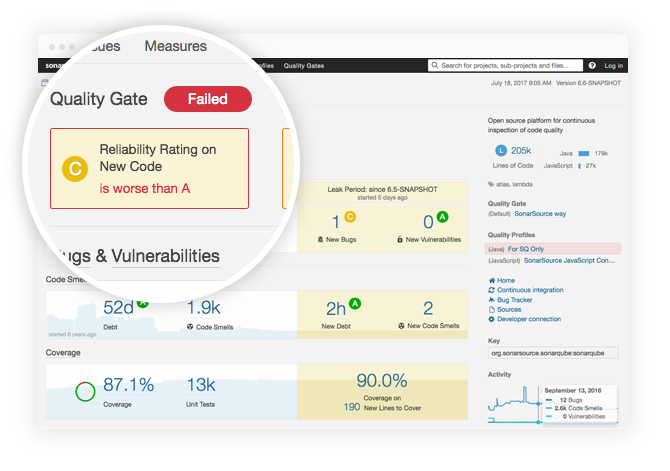
\includegraphics[width=0.9\textwidth]{images/enforce-quality-gate.png}
	\caption{dashboard con parametri di SonarQube}
	\label{qualità}
\end{figure}
\begin{figure}[!h]
	\centering
	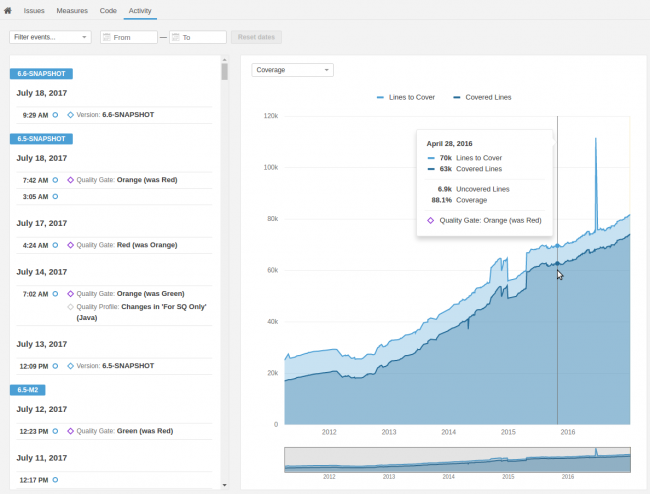
\includegraphics[width=0.7\textwidth]{images/project-history2.png}
	\caption{Grafico prodotto da SonarQube}
	\label{graficobello}
\end{figure}
\newpage
\subsection{Validazione}

\subsubsection{Scopo}
Il processo di validazione ha lo scopo di determinare se il prodotto realizzato è conforme alle attese e viene effettuato, solo quando il prodotto è completo, in seguito a molteplici verifiche per evitare di ottenere un risultato negativo.
\subsubsection{Attività}
\paragraph{Analisi dinamica} \Spazio
Il \textit{verificatore} ha il compito di rieseguire i test per la verifica per controllare che non vi siano errori non rilevati precedentemente, eseguire i test validazione per accertarsi che il prodotto sia conforme alle attese e comunicare i risultati ottenuti al \textit{project manager} che deciderà se eseguire ulteriori test.
\subsubsection{Test}
\subparagraph{Test di sistema} \Spazio
I test di sistema validano il prodotto software ovvero si accertano che rispettino i requisiti concordati, vengono effettuati quando si ritiene che il prodotto abbia raggiunto una versione definitiva.\newline
I test di sistema saranno descritti nel modo seguente: \Spazio
\centerline{\textbf{TS}[ImportanzaRequisito][TipoRequisito][idRequisito]}

dove:
\begin{itemize}
		\item \textbf{ImportanzaRequisito:} può assumere valori tra:
	\begin{itemize}
		\item 0 per i requisiti obbligatori;
		\item 1 per i requisiti desiderabili;
		\item 2 per i requisiti facoltativi.
	\end{itemize}

	\item \textbf{TipoRequisito:} può assumere valori tra:
	\begin{itemize}
		\item F per i requisiti funzionali;
		\item Q per i requisiti di qualità;
		\item V per i requisiti di vincolo;
		\item P per i requisiti prestazionali.
	\end{itemize}
	
	\item \textbf{IdRequisito:} può assumere un valore gerarchico che identifica il singolo requisito.
\end{itemize}
\subparagraph{Test di accettazione} \Spazio
Consiste nel collaudo del software in presenza del proponente, se questo test ha esito positivo il prodotto può essere rilasciato.\newline
	I test di validazione saranno organizzati nel modo seguente:\Spazio

\centerline{\textbf{TA}[ImportanzaRequisito][TipoRequisito][IdRequisito]}

dove:
\begin{itemize}
		\item \textbf{ImportanzaRequisito:} può assumere valori tra:
	\begin{itemize}
		\item 0 per i requisiti obbligatori;
		\item 1 per i requisiti desiderabili;		
		\item 2 per i requisiti facoltativi.
	\end{itemize}

	\item \textbf{TipoRequisito:} può assumere valori tra:
	\begin{itemize}
		\item F per i requisiti funzionali;
		\item Q per i requisiti di qualità;
		\item V per i requisiti di vincolo;
		\item P per i requisiti prestazionali.
	\end{itemize}
	
	\item \textbf{IdRequisito:} assume un valore gerarchico che identifica il singolo requisito.
	
\end{itemize}
